% !TEX root = ../../report.tex
\section{Hardwareaufbau}
\begin{Spacing}{\mylinespace}

Der Laboraufbau besteht aus vier Grundkomponenten, welche in Abbildung \ref{fig:laboraufbau} dargestellt sind. Die Maße der Grundfläche betragen $1m x 1m$. Der Projektor sowie die Tiefenkamera sind einen Meter über der Oberkante des Sandkastens montiert.

\vspace{0.2cm}
\textit{Rechner (Aa) inkl. Kontrollmonitor (Ab), Projektor (Ba) mit Projektionsperspektive(Bb), Tiefenkamera (Ca) mit Erfassungsperspektive (Cb), zu betrachtende Oberfläche (Sandkasten) (D)}

\begin{figure}[hbtp]
	\centering
	\label{fig:laboraufbau}
	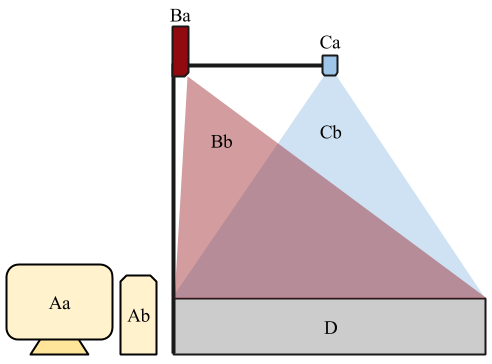
\includegraphics[width=0.6\textwidth]{graphics/Aufbau.png}
	\caption{Laboraufbau}
\end{figure}

\subsection{Rechner}

Verwendet wurde der zur Verfügung gestellte Laborrechner von Fujitsu Siemens. Er verfügt über zwei Intel Xenon Prozessoren. Die Grafikleistung wurde von einer, speziell für diesen Aufbau angeschafften, NVIDIA GeForce GT780. Zur Kontrolle, als auch für Konfigurationszwecke wurde noch ein Kontrollmonitor begestellt. Der Projektor sowie die Tiefenkamera sind beide mit dem Rechner verbunden.

\subsection{Projektor}

Nach dem die ersten Versuche mit einem älteren BenQ Projektor getätigt wurde kam im weitern Verlauf ein Projektor der Firma Optoma vom Typ X306 ST zum Einsatz. Durch die hohe Lichtstärke von 3200 Ansi Lumen konnte eine gute Darstellung realiesiert werden. Die Befestigung erfolgte Kopfüber. Durch Stellschrauben an der Vorrichtung, kann nachträglich eine Kalibrierung mit dem Sandkasten erfolgen.

\subsection{Tiefenkamera}

Zur Erfassung der Höheninformation der Oberfläche wurde die Tiefenkamera Kinect for Windows von der Firma Microsoft verwendet. Sie arbeitet nach dem Prinzip des Structured-Light-Coding und besitzt eine Höhengenauigkeit von einem Millimeter. 

\begin{figure}[hbtp]
	\centering
	%Bild oben
	\subfloat[Kinect Hardware]{
	\label{fig:kinHW}
	\inputTikZ{graphics/kinectHW}
	}
	\hfill
	% Bild unten
	\subfloat[Kinect Sichtfeld im Nahmodus]{
	\label{fig:fov}
	\inputTikZ{graphics/fov}
	}
	\caption{Kinect Sensor}
\end{figure}


\subsection{Sandkasten}

Was das mit dem Sand war\\

\end{Spacing}
\newpage
\clearpage
%% End Of Doc